\chapter{Smart Home Viewer}
Smart Home Viewer est une application de télémaintenance permettant de faire le diagnostique de la connexion internet d'un modem internet.
\begin{figure}[H]
	\centering
	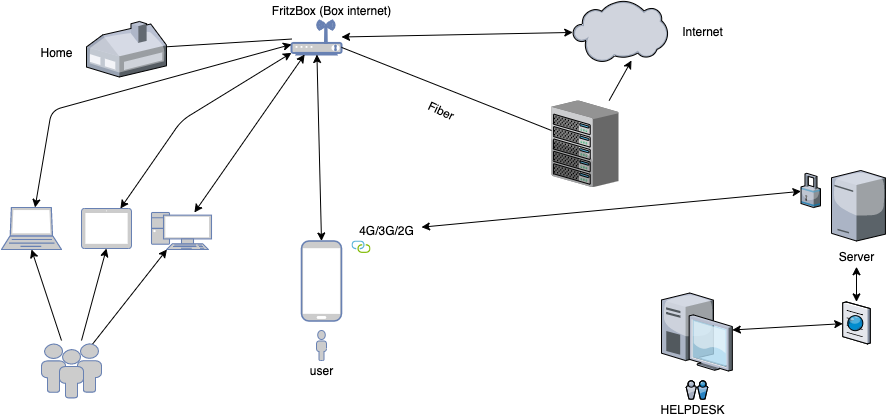
\includegraphics[scale=0.4]{assets/images/shv.png}
	\caption{Description global du système de fonctionnement de l'application}
	\label{fig.3}
\end{figure} 
Le contexte de fonctionnement de l'application est lorsque pour une raison ou une autre, un utilisateur de la box de l'entreprise voit sa connexion internet s'interrompre. Dans ce cas, il appelle le centre d'appel de l'entreprise et l'operateur lui fournit un code de connexion pour le diagnostique de sa connexion.

Le processus de diagnostique de la connexion est décrit sur la figure \ref{fig.3}. Pour faire fonctionner l'application, l'utilisateur devra activer son Wifi et ses données mobiles. La liaison Wifi servira à la communication avec la box et les données mobiles serviront à envoyer les données de la box au serveur.

Lorsque l'utilisateur s'authentifie avec le code que l'opérateur lui a fourni, l'opérateur, le téléphone est prêt pour servir de canal de transmission de l'information entre la box et le serveur. L'opérateur déclenche la communication entre les appareils puis le serveur envoie les requêtes nécessaires à la box pour récupérer et afficher la page d'accueil de la box directement sur le poste de l'opérateur qui pourra vérifier les paramètres et faire des modifications si nécessaire.

Dans la suite, il sera décrit le fonctionnement du système.
\section{Contexte du système}
Dans cette section je présente le diagramme de contexte du système afin de localiser l'application dans son environnement. Il est aussi décrit les acteurs qui interagissent avec le système. Dans la suite de ce chapitre, \textit{Modem} fait référence à la box.
\begin{figure}[H]
	\centering
	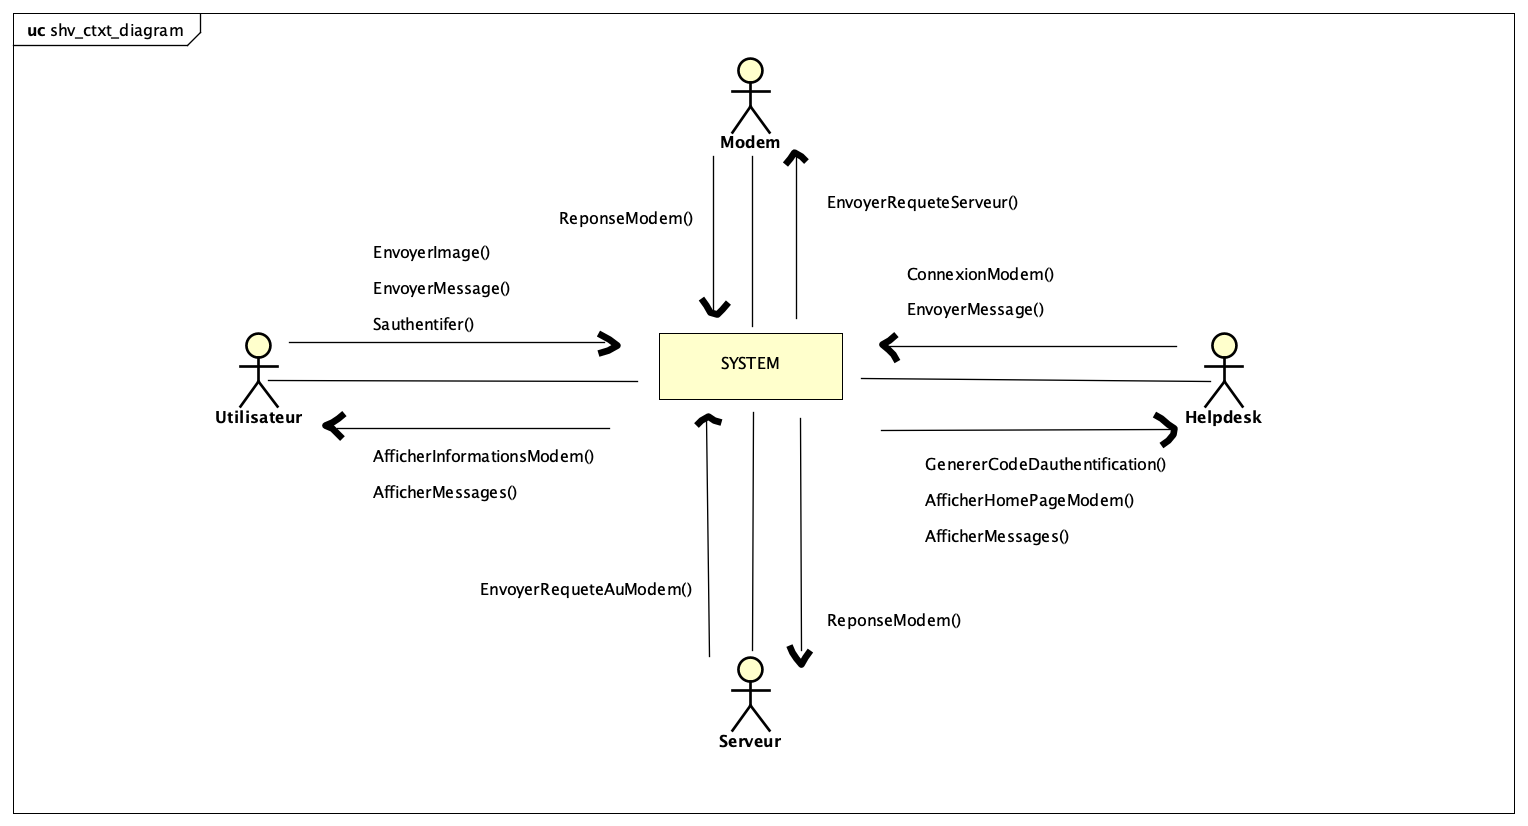
\includegraphics[scale=0.4]{assets/images/shv_ctxt.png}
	\caption{Diagramme de contexte}
	\label{fig.4}
\end{figure} 

\emph{L'utilisateur} et le \hd sont les acteurs principaux du système. Afin d'initier la communication, le \hd doit fournir le code d'authentification à l'utilisateur. Le code d'authentification est généré par le système côté serveur et fourni au \hd. \textit{GenererCodeDauthentification()} consiste à générer un code à six chiffres, l'associer à une session et à l'afficher au \hd. L'\emph{utilisateur} se connecte au système via ce code. Il réalise cette connexion via \textit{Sauthentifier()}. Une fois authentifier, le système côté client effectue quelques requêtes afin d'afficher à l'utilisateur, les informations de son Modem. Les informations sont affichées via \textit{AfficherInformationsModem()}. Le \hd et l'\emph{utilisateur} peuvent s'échanger via un chat et les fonctions principales de ce chat est l'envoie des messages et d'images. Ces fonctions sont réalisées via \textit{EnvoyerMessage()}, \textit{EnvoyerImage()} et \textit{AfficherMessages()}.

 Une fois la connexion réalisée par l'\emph{utilisateur}, le \hd, peut déclencher l'affichage de la page d'accueil du modem. Si la requête est fait, le serveur envoie et reçoit des requêtes au système via les fonctions \textit{EnvoyerRequeteAuModem()} et \textit{ReponseModem()}. Le système récupère la requête du serveur, construit une nouvelle requête spécifique et l'envoie au modem qui répond au système en retour en fonction des éléments demandés. Les fonctions misent à contributions sont \textit{EnvoyerRequeteServeur()} et \textit{ReponseModem()}. Si tout se passe bien, le serveur construit à partir des éléments fournis par le modem la page d'accueil du modem et l'affiche au \hd.
 
Du point de vue du fonctionnement du système, les acteurs \emph{Modem} et \emph{Serveur} sont certes secondaires mais indispensable. C'est la connexion internet du modem qui est diagnostiquée. Le serveur a pour rôle de servir d'interface pour le \hd et de serveur pour l'application du point de vue de l'architecture client-serveur pour une application. Le système sert donc d'intermédiaire ou de moyen de communication entre le \emph{modem} et le \emph{serveur}.

\section{Caractéristique de l'utilisateur}
L'application est destinée à l'utilisation des clients de la société \lol ayant souscris à une offre internet via box ou ADSL. L'utilisation de l'application ne requiert aucune compétence particulière à part le fait de savoir utiliser un smartphone.

\section{Contraintes principaux de développements}
L'application a été développé pour les deux plateformes mobiles Android et iOS et selon le paradigme orienté objet. Pour ce faire j'ai utilisé le langage de programmation Java\footnote{Java est un langage de programmation objet créé par Sun microsystems et détenu depuis 2009 par Oracle. }, l'environnement de  développement d'application Android et l'IDE Android Studio pour l'application Android et le les langages Swift\footnote{Swift est un langage de programmation objet, multiparadigme, open-source développé par Apple en 2014 } et Objective C\footnote{Objective C est un langage orienté objet réflexif créé en 1983 et détenu par Apple.} avec l'environnement de développement d'application Cocoa Touch et l'IDE XCode pour l'application iOS. 

J'ai aussi utilisé des standards RFC pour des questions réseaux.

\section{Besoins fonctionnels}
Il s'agit ici de décrire les besoins fonctionnels du système à travers les cas d'utilisation de l'application.
\subsection*{Description générale}
Le diagramme de la figure \ref{fig.4} présente une vue générale des cas d'utilisations du système. Chaque cas d'utilisation lié à un acteur, décrit un état atteint par le système au cours de l'exécution de l'application. Au cours des prochaines sections, je détaillerai plus précisément les cas d'utilisation en les décomposant par acteur.
\begin{figure}[H]
	\centering
	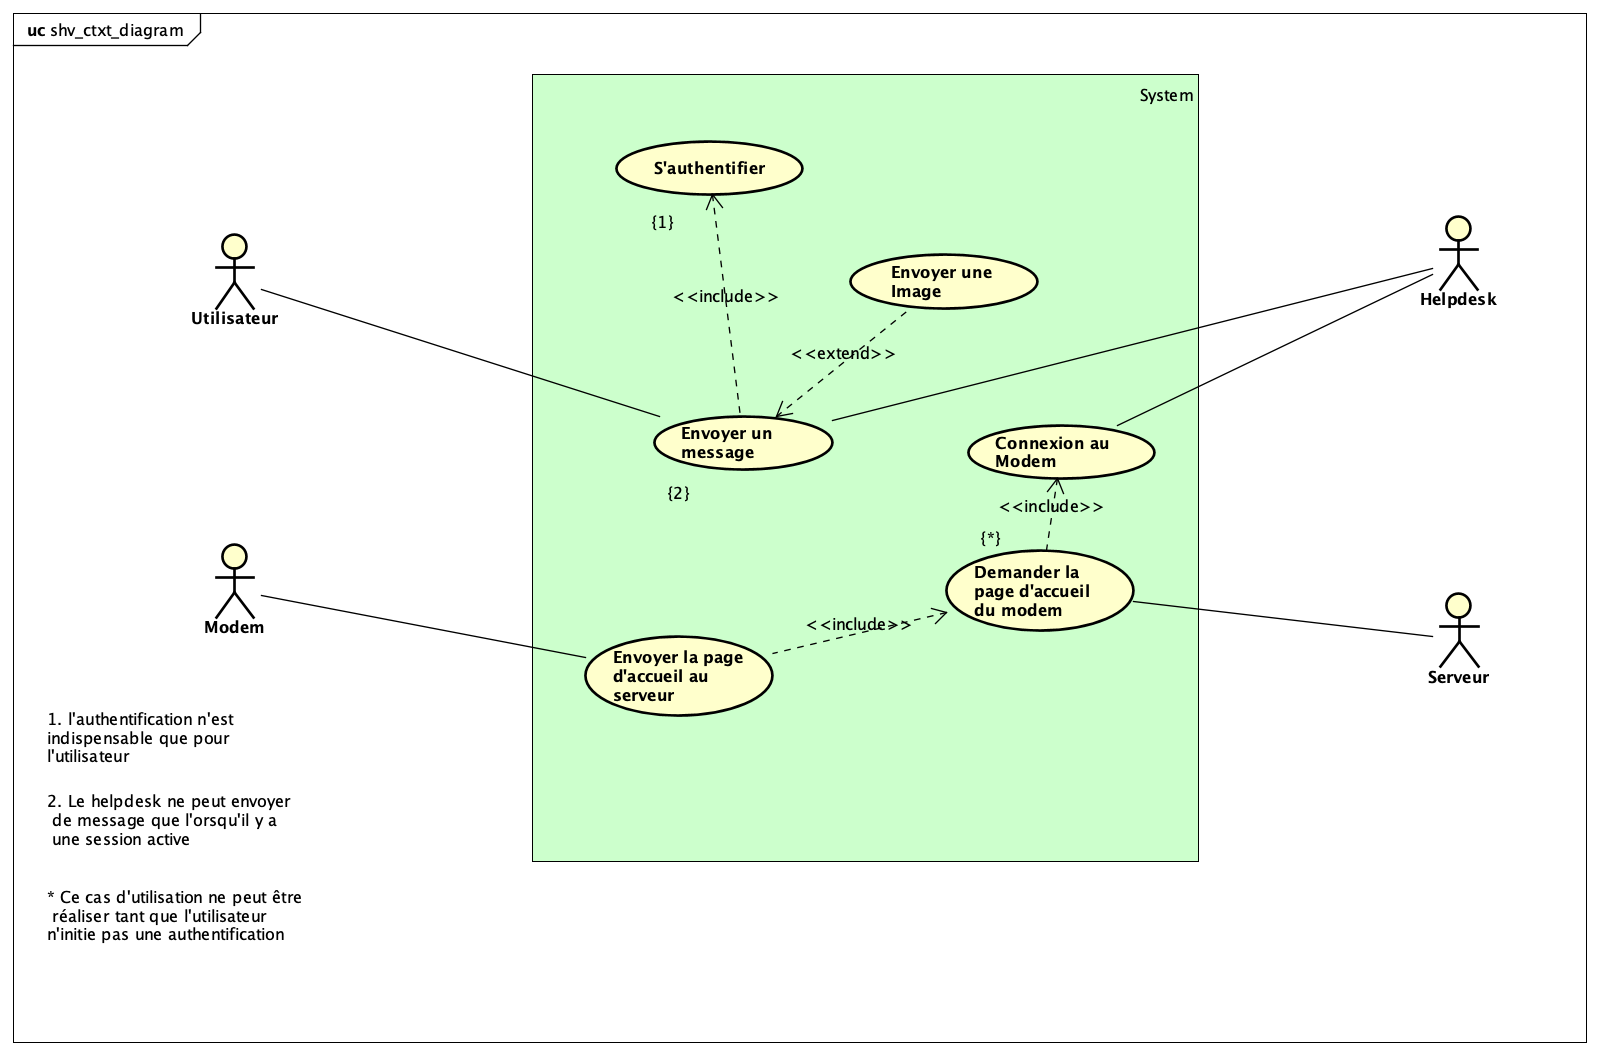
\includegraphics[scale=0.4]{assets/images/shv_use_case.png}
	\caption{Diagramme de cas d'utilisation}
	\label{fig.5}
\end{figure}

\subsection{Description des cas d'utilisations par acteur}
Le système est composé de quatre acteurs principaux à savoir l'\ut, le \hd, le \md et le \sv. Pour comprendre totalement le rôle joué par chacun, je procède ici à une briève description de chacun d'eux.
\subsubsection*{L'utilisateur}
Le principal rôle de l'\ut est de se créer une session en s'authentifiant sur l'application. Il pourra envoyer un message ou l'image de son appareil au \hd. Il pourra aussi lire les messages envoyés par le \hd.

\subsubsection*{Le helpdesk}
Les principaux rôles du \hd sont de générer le code d'authentification à l'\ut en démarrant la session et de se connecter au \md. Il pourra aussi fermer la session de l'\ut ou encore envoyer et lire les messages de ses échanges avec l'\ut.

\subsubsection*{Le modem}
Le \md est l'appareil qui est diagnostiqué. Son rôle dans le fonctionnement du système est de recevoir, traiter et répondre aux requêtes envoyer par le serveur via le système.

\subsubsection*{Le Serveur}
Les principaux rôles du \sv sont de créer et clore la session pour l'utilisateur, construire les requêtes à envoyer au \md et envoyer les messages.

\subsection{Description des cas d'utilisation}
\subsubsection*{Description du cas d'utilisation de connexion à l'appareil}
\begin{enumerate}
	\item[]\underline{Résumé d'identification}
		\begin{itemize}
			\item[]Titre : Connexion au modem
			\item[]Résumé: Initier la communication entre le serveur et le modem et début du diagnostique.
			\item[]Acteurs: \hd (principal), \md, \sv
			\item[]Date de création: 23 Septembre 2019
			\item[]Date de mise à jour: 25 Septembre 2019
			\item[]Version: 1.0
			\item[]Description des scénarii
			\item[]Pré-condition:
			\begin{itemize}
				\item L'\ut s'est authentifié et la session a été démarrée
				\item L'\ut a activé le wifi et les données mobile sur son téléphone et le wifi est connecté au modem à diagnostiquer. 
			\end{itemize}
			\item[]\underline{Scénarii nominaux}
			\begin{enumerate}
				\item[1.] Le \hd démarre la connexion au modem.
				\item[2.] La connexion entre le \sv et le  \md a été effectuée avec succès et la communication est déclenchée (A1)
				\item[3.] La page d'accueil du modem est affichée dans un nouvel onglet dans le navigateur web du \hd
			\end{enumerate}
			\item[]\underline{Scénario alternatif}\\
			A1 : Ce scénario est déclenché lors du point 2 des scénarii nominaux lorsque pour une raison la connexion est interrompue.
			
			Le système réinitie la communication en trois tentative.
			\item[]\underline{Scénario d'exception}\\
			E1: Ce scénario est déclenché en A1 lorsque après trois tentatives de réinitialisation de la communication, la liaison est toujours cassée entre le \md et le \sv.
			
			Le système déconnecte l'utilisateur et demande à nouveau le code d'authentification.
			
			\item[]\underline{Post-condition:}
			\begin{itemize}
				\item La page d'accueil du modem est affichée
				\item La session reste active
			\end{itemize}
		\end{itemize}
\end{enumerate}
\section{Spécification des structures de données}
Au cours de cette section, les diagrammes de classes ne concernent que la version Android de l'application mais les fonctionnalités sont les mêmes sur les deux versions de l'application.

\subsection{Module de communication}
Pour réaliser la communication entre les différentes entités intervenant dans l'exécution de l'application, j'ai utilisé les \textbf{Socket} au niveau logiciel. Ainsi pour ce faire, j'ai appliqué le design pattern factory pour créer deux classes dans un contexte orienté objet à savoir \textsl{ModemSocket} et \textsl{ServeurSocket} afin de définir le comportement au niveau de l'application des interfaces de communication du \sv et du \md.
\begin{figure}[H]
	\centering
	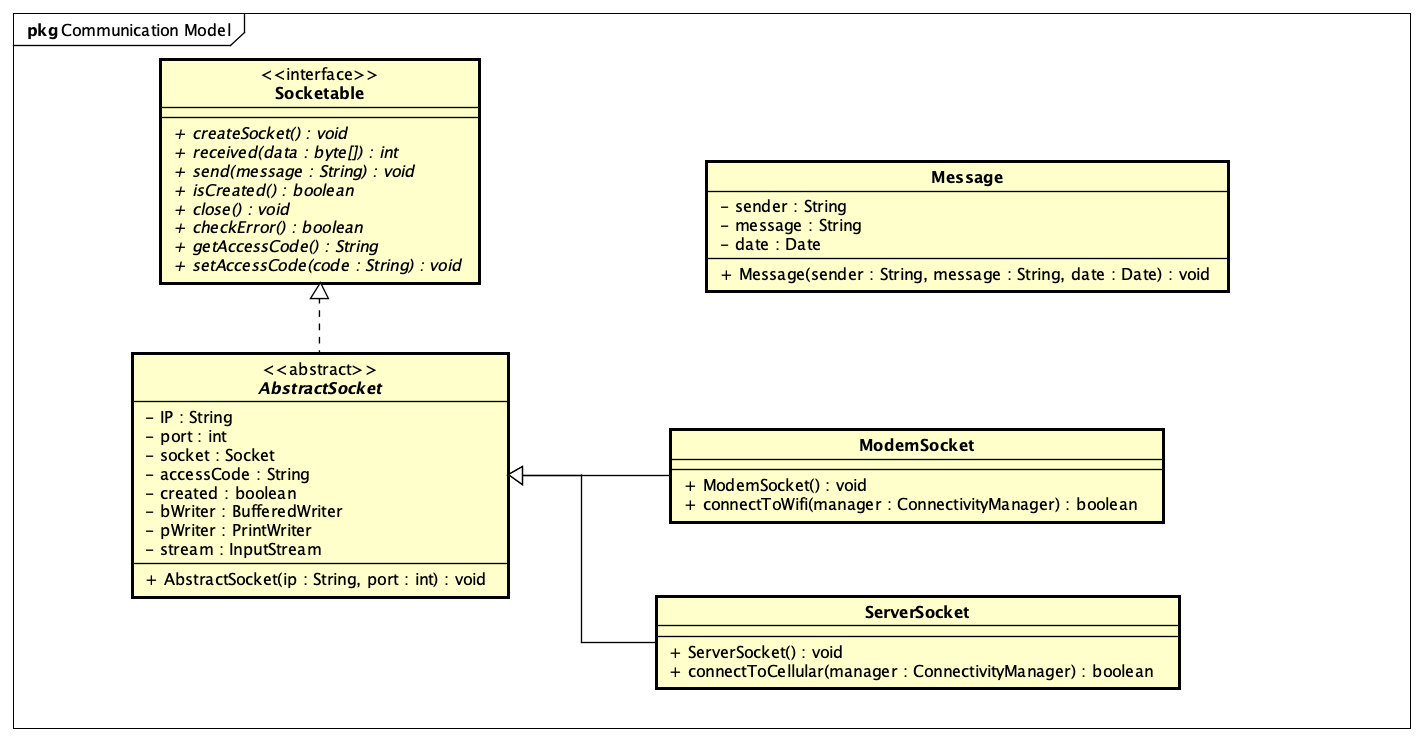
\includegraphics[scale=0.4]{assets/images/shv_communication_cd.png}
	\caption{Diagramme de classe du module de communication}
	\label{fig.6}
\end{figure}

Au lancement de l'application, un service au sens programmation, est démarré. Ce service possède les méthodes nécessaires pour authentifier et établir la connexion entre le \sv et le \md. Le diagramme de classe des services est présenté en annexe.

Dans la suite est présenté le diagramme d'activité représentant comment est géré la communication au niveau de l'application.

\begin{figure}[H]
	\centering
	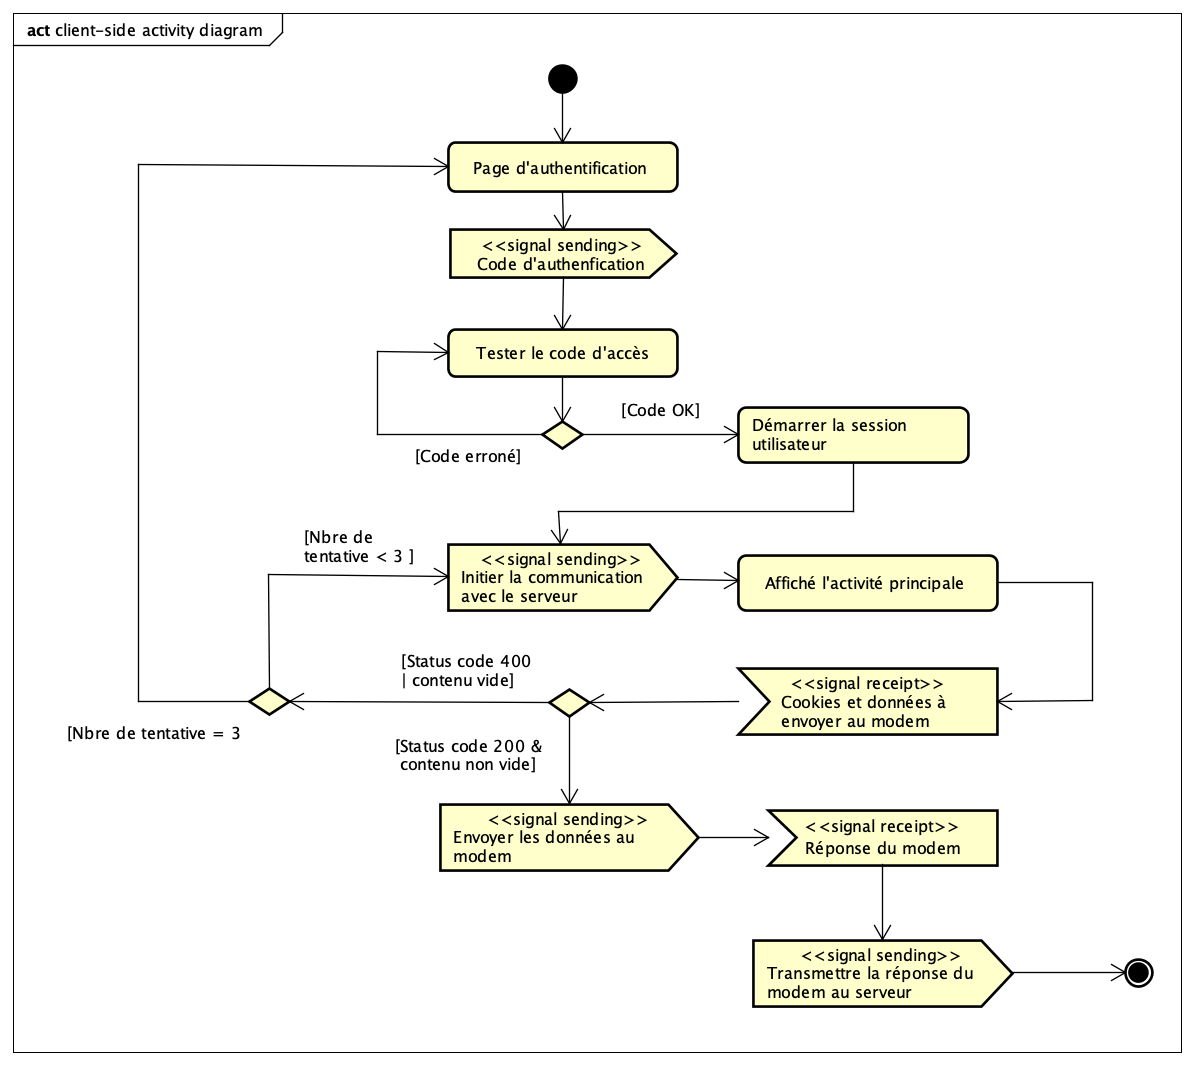
\includegraphics[scale=0.4]{assets/images/client_side_activity_diagram.png}
	\caption{Diagramme d'activité du module de communication}
	\label{fig.7}
\end{figure}
Comme décrit sur la figure \ref{fig.7}, la communication est réalisée via  le protocole HTTP. Ainsi une fois la session démarrée, le fonctionnement du système est lié à la bonne réception des données de la part du service de l'application et du serveur. Si le code de statut HTTP est 200, la communication est effective mais s'il est 400 le service réinitie la communication jusqu'à trois fois. Si après trois tentatives le service ne reçoit toujours pas un code 200, la communication est interrompu au niveau du programme et l'\ut est redirigé vers la page d'authentification.

\section{Spécification des interfaces externes}
\subsection{Interface Matériel/logiciel}
\subsubsection*{Configuration minimale sur laquelle le système peut s'exécuter}
Pour faire fonctionner l'application sur un appareil mobile, l'appareil devra avoir les configurations minimales suivantes :
\begin{itemize}
	\item Matériel : Tous les smartphones android ou iOS supportant les configurations minimales au niveau logiciel.
	\item Logiciel : Tous les smartphones android supportant au moins la version 5.0 (Android Lollipop) ou les smartphones iOS supportant au moins la version 12.0 d'iOS.
\end{itemize}

\subsubsection*{Protocole d'échange}
Pour le fonctionnement du système les protocoles utilisés sont le HTTP et un protocole développé par l'entreprise.

\subsection{Interface logiciel/logiciel}
Pour développer l'application, les outils suivants ont été utilisés:
\begin{itemize}
	\item lanagages et bibliothèques de développement 
	\begin{itemize}
		\item[-] Java 1.8
		\item[-] Swift 5.1
		\item[-] Objective C 2.0
		\item[-] Gradle 5.4.1
		\item[-] Android API 29
		\item[-] Cocoa Touch Framework 
	\end{itemize}
	\item Outils de développement
	\begin{itemize}
		\item[-] Android Studio 3.5
		\item[-] XCode 10.0
		\item[-] Git 2.2
		\item[-] GitLab
		\item[-] Mac Mini 2019 et MacOS Mojave
		\item[-] Samsung Tab 4
		\item[-] iPad mini 2
	\end{itemize}
\end{itemize}

\subsection{Interface homme-machine}
\subsubsection*{Structure}
\begin{figure}[H]
	\centering
	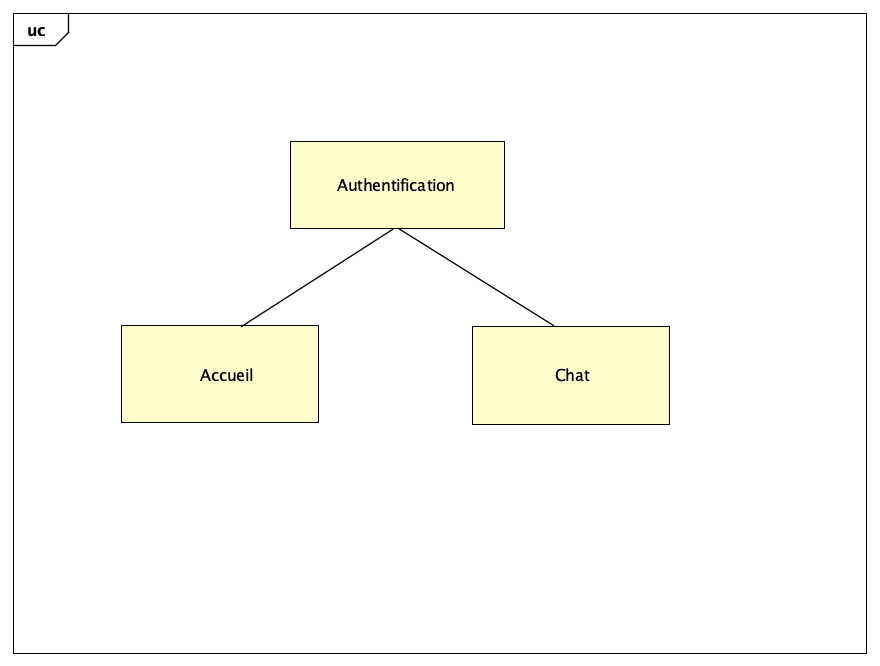
\includegraphics[scale=0.4]{assets/images/ihm.png}
	\caption{Structure IHM de l'application}
	\label{fig.8}
\end{figure}
\section{Déroulement du stage}
\subsection{Développement et difficultés rencontrés}
Le développement de l'application Smart Home Viewer a été commencé en 2016 par un ancien stagiaire mais il n'a pas pu le terminé avant son départ. Lorsque j'ai repris le code, j'ai dû lire l'intégralité de son code et le compilé pour savoir exactement ce que je dois améliorer ou ajouter. Le code compilait mais l'application ne fonctionnait pas. J'ai d'abord refactoré le code, changé d'architecture et ajouté des fonctionnalités pour qu'elle fonctionne. Je dois dire que malgré le fait que l'application ne fonctionnait pas l'ancien stagiaire m'avait mâché le travail.

J'ai d'abord pris en main l'application android et après l'avoir fait fonctionné totalement, j'ai réimplémenté les mêmes choses sur la version iOS.

Les premières difficultés sont apparus lors des premiers tests. En effet il arrivait que des fois la communication entre les appareils s'interrompaient inopinément ou encore après quelques minutes d'inactivité, la session se terminait tout seul.

Pour résoudre ces problèmes, j'ai mis en place un mécanisme basé sur le pattern Observer pour reconnecter automatiquement les appareils. Si après trois tentatives la reconnexion ne fonctionne pas, la session de l'\ut est déconnectée automatiquement.

Pour résoudre le problème qui survient à cause de l'inactivité, nous avons mis en place un protocole semblable a du ping pong pour garder la session active.

Le diagramme du modèle observateur que j'ai implémenté est disponible dans l'annexe.